\documentclass[a4paper]{article}

\usepackage[T2A]{fontenc}
\usepackage[utf8]{inputenc}
\usepackage[russian]{babel}
\usepackage{graphicx}
\usepackage{float}
\usepackage{mathtools}
\usepackage{wrapfig}
\usepackage{amsfonts, amssymb, amsmath, latexsym}
\usepackage{nicefrac}
\usepackage{hhline}
\usepackage{multirow}
\usepackage[colorlinks=true,linkcolor=blue,citecolor=blue]{hyperref}       % hyperlinks
\usepackage{nicefrac}       % compact symbols for 1/2, etc.
\usepackage{nameref}
\usepackage{booktabs}       % professional-quality tables
\usepackage{algorithm}
\usepackage{algpseudocode}
\usepackage{xcolor, colortbl}
\usepackage{etoolbox}

% \graphicspath{ {./} }

\usepackage[verbose=true,letterpaper]{geometry}

\newgeometry{
    textheight=25cm,
    textwidth=18cm,
    top=2.5cm,
    headheight=12pt,
    headsep=25pt,
    footskip=1cm,
    marginparwidth=15pt
}

%\usepackage{showframe} 

\usepackage{epigraph}
\usepackage{amsmath,amsfonts,amssymb,amsthm,mathtools, mathrsfs}
\usepackage{amsthm}

\title{Работа 4.3.4 \\ Преобразование Фурье в оптике}
\author{Шарапов Денис, Б05-005}
\date{}

\usepackage{fancyhdr}
\pagestyle{fancy}
\fancyhf{}
\rhead{Работа 4.3.4}
\lhead{}
\cfoot{\thepage}
\usepackage{subcaption}
\usepackage[font={small}]{caption}

\begin{document}

    \maketitle
    \tableofcontents
    \newpage
    
\section{Аннотация}

\noindent\textbf{Цель работы:} наблюдение дифракционной картины и ее исследование с точки зрения разложения в ряд Фурье. \smallskip
 
\noindent \textbf{В работе используются:} гелий-неоновый лазер, кассета с набором сеток разного периода, щель с микрометрическим винтом, линзы, экран, линейка.

\section{Результаты измерений и обработка данных}

\subsection{Определение ширины щели}

\begin{figure}[ht!]
    \centering
    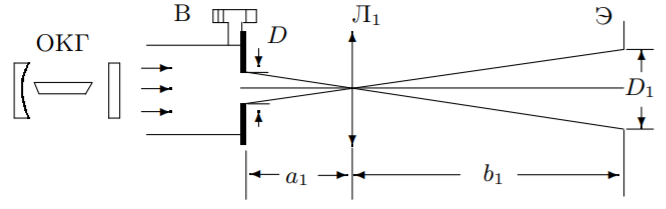
\includegraphics[width = 0.7\textwidth]{image/scheme1.png}
    \caption{Схема для определения ширины щели с помощью линзы, где $a_1 = 26$ см, $b_1 = 130$ см, $F_1 \approx 3-4$ см, Л$_1$ -- линза с фокусным расстоянием $F_1$, Э -- экран, $D$ -- ширина щели, $D_1$ -- размер изображения}
\end{figure}

Установим тубус со щелью вплотную к выходному окну лазера (рис. 1). С помощью короткофокусной линзы~Л$_1$ получим на экране Э увеличенное изображение щели. Меняя ширину щели, снимем зависимость размера изображения $D_1$ от ширины щели $D$ (табл. 1). По полученной таблице построим график искомой зависимости:

\begin{figure}[h!]
    \centering
    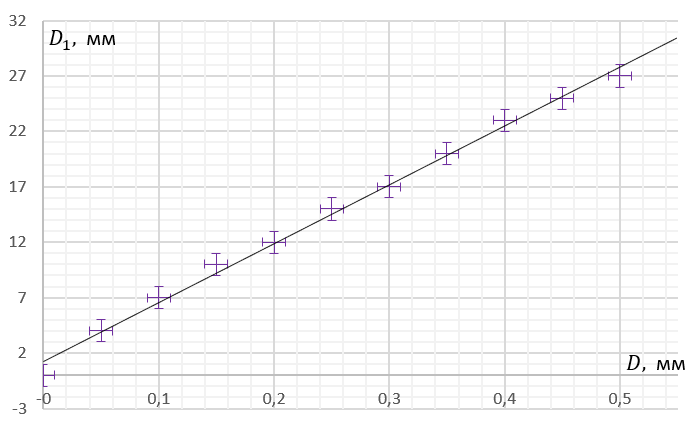
\includegraphics[width = 0.7\textwidth]{image/graph1.png}
    \caption{График зависимости размера изображения $D_1$ от ширины щели $D$}
\end{figure}

\noindent Из графика получим значение $\Gamma$:
$$\Gamma = 51,4 \pm 1,1,$$ которое в пределах погрешности совпадает со значением 
$$\Gamma = \frac{b_1}{a_1} = 50,0 \pm 1,5.$$

\subsection{Определение ширины щели по её спектру}

Получим на удалённом экране пектр щели (рис. 3). Проведём серию измерений $X(m)$, меняя ширину щели в тех же пределах, что и в пункте 2.1.
\begin{figure}[h!]
    \centering
    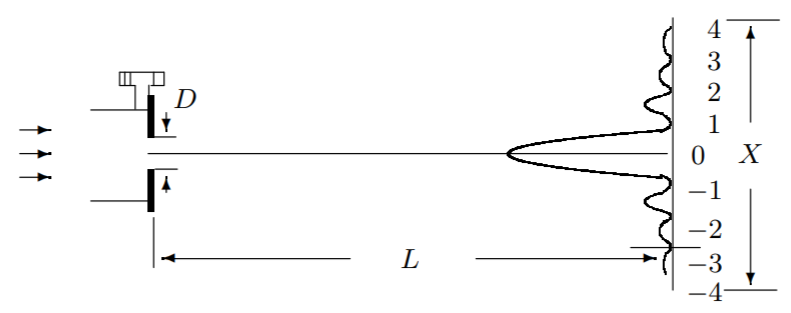
\includegraphics[width = 0.7\textwidth]{image/scheme2.png}
    \caption{Схема для определения ширины щели по спектру, где $L = 131$ см -- расстояние от щели до экрана}
\end{figure}

\noindent По результатам измерений спектра рассчитаем ширину щели $D_c$, используя соотношения
$$\Delta X = \frac{X}{2m} = \frac{\lambda}{D_c}L.$$ Полученные результаты представлены в таблице 2. График зависимости $D_c = f(D)$ представлен на рис. 4.

\begin{figure}[h!]
    \centering
    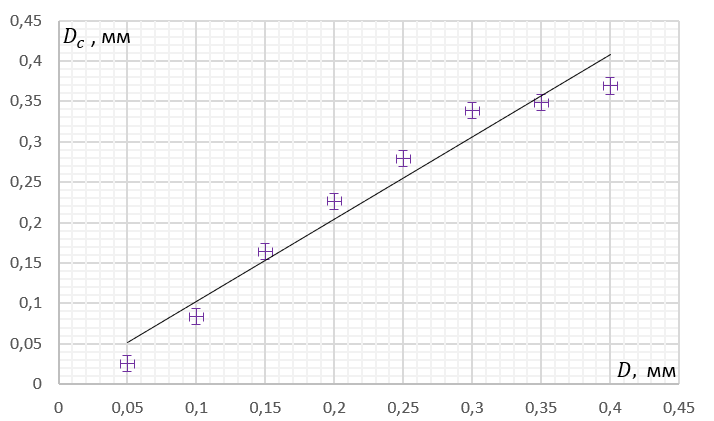
\includegraphics[width = 0.7\textwidth]{image/graph2.png}
    \caption{График зависимости ширины щели $D_c$ (<<c>> -- по спектру) от ширины щели $D$}
\end{figure}

\subsection{Определение периода решёток по спектру на удалённом экране}

Поставим кассету с двумерныи решётками вплотную к выходному окну лазера. Для каждой сетки измерим расстояние $X$ между $m$-ми максимумами и отметим $m$ --- порядок максимума. Рассчитаем расстояния $\Delta X$ между соседними максимумами и определим период решётки $d_c = f(\text{№})$, используя соотношения
$$\Delta X = \frac{X}{2m} = \frac{\lambda}{d_c}L.$$
Результаты приведены в таблице 3.

\subsection{Определение периода решёток по увеличенному изображению спектра}

Линзу Л$_2$ с максимальным фокусом $F_2$ поставим на расстоянии $\approx F_2$ от кассеты (рис 5). В плоскости $\Phi$ линза Л$_2$ даёт фурье-образ сетки --- её спектр, а короткофокусная линза Л$_3$ создаёт на экране увеличенное изображение этого спектра. 

\begin{figure}[h!]
    \centering
    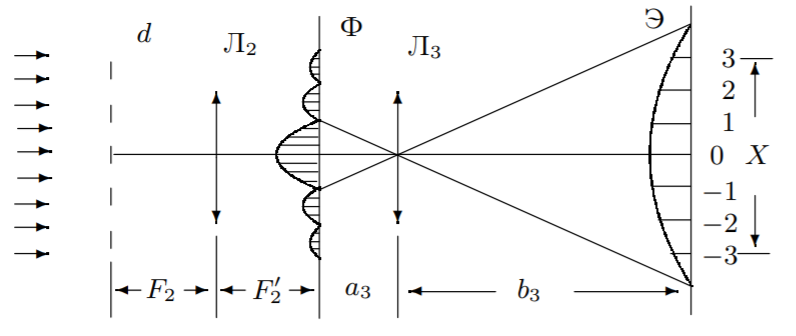
\includegraphics[width = 0.7\textwidth]{image/scheme3.png}
    \caption{Схема определения периода решётки по увеличенному изображению спектра, где $a_3 = 30$ см, $b_3 = 100$ см, $F_3 \approx 2,5$~см -- фокус линзы Л$_3$, $F_2 \approx 10$ см -- фокус линзы Л$_2$, Ф -- фокальная плоскость линзы Л$_2$}
\end{figure}


\noindent Измерим $X$ и $m$ для всех сеток, где это возможно. Результаты внесём в таблицу 3.

\subsection{Мультиплицирование}

Поставим тубус со щелью к окну лазера и найдем на экране резкое изображение с помощью линзы Л$_2$ (рис). В фокальной плоскости Ф линзы Л$_2$ поставим кассету с сетками, которые будут <<рассекать>> фурье-образ щели --- осуществлять пространственную фильтрацию.

\begin{figure}[h!]
    \centering
    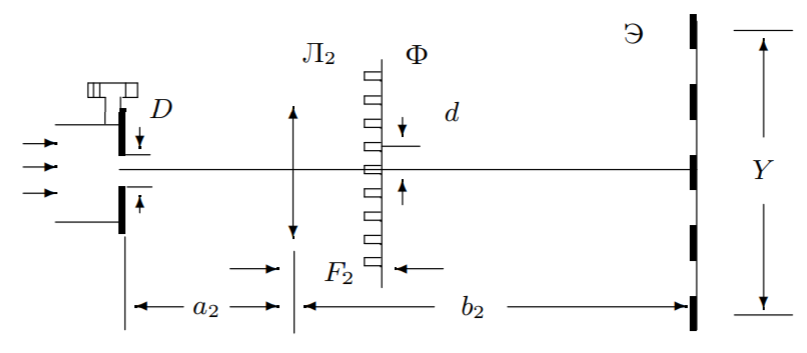
\includegraphics[width = 0.7\textwidth]{image/scheme4.png}
    \caption{Схема для наблюдения мультиплицирования, где $a_2 = 10$ см, $b_2 = 130$ см, $Y$ --- расстояние между удаленными изображениями щели}
\end{figure}

\noindent Рассчитаем периоды $\Delta y$ <<фиктивных>> решёток, которые дали бы такую же периодичность на экране: $$\Delta y = \frac{\Delta Y}{\Gamma_2},$$ где $$\Delta Y = \frac{Y}{K}$$ и $K$ --- число промежутков между изображениями. Результаты приведены в таблице 4. \medskip

\noindent Построим график $\Delta y = f(1/d_c)$, где $d_c$ --- периоды решёток, определённые по спектру. Зависимость должна быть линейной, поскольку 
$$\frac{\lambda}{\Delta y}F_2 = d_c.$$ \newpage

\begin{figure}[h!]
    \centering
    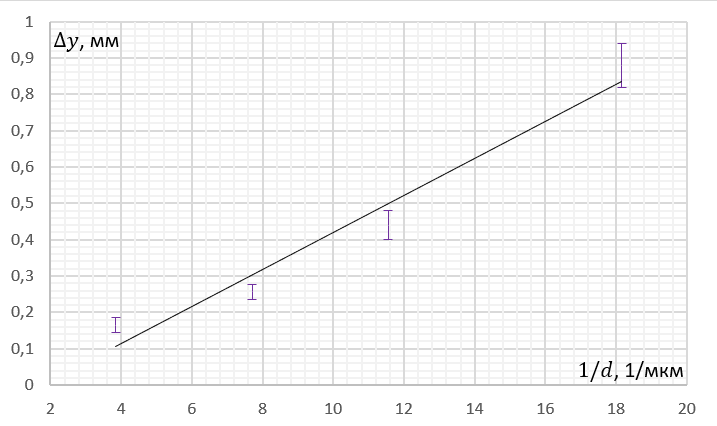
\includegraphics[width = 0.7\textwidth]{image/graph3.png}
    \caption{График зависимости периода $\Delta y$ <<фиктивных>> решёток от периодов решёток $d_c$, определённых по спектру}
\end{figure}

\section{Вывод}

В работе наблюдалась и исcледовалась дифракционная картина с точки зрения разложения в ряд Фурье. Сперва двумя способами была определена ширина щели: прямым способом (с помощью линз) и по спектру щели. В обоих случаях наблюдается линейная зависимость (рис. 2 и 4). После чего был определён период решёток двумя способами: по спектру на удалённом экране и по увеличенному изображению спектра. Результаты, приведённые в табл. 3, показывают, что эти два метода измерения дают очень близкий результат. В заключении было проведено мультиплицирование: была получена зависимость <<фиктивных решёток>> $\Delta y$ от периодов решёток $d$, причём она оказалась линейной, что подтверждает теорию.

\section{Приложение: таблицы}

\begin{table}[h!]
    \centering
    \caption{Зависимость размера изображения $D_1$ от ширины щели $D$}
    \begin{tabular}{|c|c|}
    \hline
    $D$, мм & $D_1$, мм \\ \hline
    0,00    & 0,00      \\ \hline
    0,05    & 4,00      \\ \hline
    0,10    & 7,00      \\ \hline
    0,15    & 10,00     \\ \hline
    0,20    & 12,00     \\ \hline
    0,25    & 15,00     \\ \hline
    0,30    & 17,00     \\ \hline
    0,35    & 20,00     \\ \hline
    0,40    & 23,00     \\ \hline
    0,45    & 25,00     \\ \hline
    0,50    & 27,00     \\ \hline
    \end{tabular}
    \end{table}

\newpage

    \begin{table}[h!]
        \centering
        \caption{Зависимость ширины щели $D_c$ от ширины щели $D$}
        \begin{tabular}{|c|c|c|}
        \hline
        $m$ & $X$, мм & $D_c$, мм \\ \hline
        2   & 110     & 0,025     \\ \hline
        6   & 100     & 0,083     \\ \hline
        12  & 102     & 0,163     \\ \hline
        13  & 80      & 0,226     \\ \hline
        16  & 80      & 0,278     \\ \hline
        17  & 70      & 0,338     \\ \hline
        15  & 60      & 0,348     \\ \hline
        9   & 34      & 0,368     \\ \hline
        \end{tabular}
        \end{table}


    \begin{table}[h!]
        \centering
        \caption{К определению периода решёток по спектру и по увеличенному изображению спектра}
        \begin{tabular}{|c|c|c|c|c|c|c|c|c|}
        \cline{1-4} \cline{6-9}
        № & $m$ & $X$, мм & $d_c$, мкм &  & № & $m$ & $\Delta X$, мм & $d_{\text{л}}$, мкм \\ \cline{1-4} \cline{6-9} 
        1 & 3   & 40  & 0,097    &  & 1 & 3   & 40         & 0,011    \\ \cline{1-4} \cline{6-9} 
        2 & 7   & 165 & 0,055    &  & 2 & 7   & 165        & 0,048    \\ \cline{1-4} \cline{6-9} 
        3 & 1   & 15  & 0,086    &  & 3 & 1   & 15         & 0,084    \\ \cline{1-4} \cline{6-9} 
        4 & 1   & 10  & 0,129    &  & 4 & 1   & 10         & 0,117    \\ \cline{1-4} \cline{6-9} 
        5 & 1   & 5   & 0,259    &  & 5 & 1   & 5          & 0,251    \\ \cline{1-4} \cline{6-9} 
        \end{tabular}
        \end{table}

        \begin{table}[h!]
            \centering
            \caption{Зависимость периодов $\Delta y$ <<фиктивных>> решёток от периодов решёток, определённых по спектру}
            \begin{tabular}{|c|c|c|c|c|c|c|c|}
            \hline
            № & $m$ & $X$, мм & $d$ мкм & $Y$, мм & $K$ & $1/d$, 1/мкм & $\Delta y$ \\ \hline
            1 & 3   & 40      & 0,097   & 80      & 5   & 10,27        & 1,23       \\ \hline
            2 & 7   & 165     & 0,055   & 80      & 7   & 18,15        & 0,87       \\ \hline
            3 & 1   & 15      & 0,086   & 40      & 7   & 11,55        & 0,43       \\ \hline
            4 & 1   & 10      & 0,129   & 20      & 6   & 7,70         & 0,25       \\ \hline
            5 & 1   & 5       & 0,259   & 15      & 7   & 3,85         & 0,16       \\ \hline
            \end{tabular}
            \end{table}


\end{document}